\documentclass{article}
\usepackage[utf8]{inputenc}
\usepackage{graphicx}

\title{Image Processing : Assignment-1}
\author{Digdarshan Kunwar, Eaindra Wun Pyae}
\date{February 2021}

\begin{document}

\maketitle

\section{Erosion}
\subsection{Erosion of f1 by square of size 3}
Considering the center of the SE (3 $\times$ 3) as the origin (0,0), a padding of 1 is added to all borders of f1 as indicated below as 'img\_with\_boundary'. Since f1 is saved in the binary format, we have to check whether all 8 neighbors of each pixel of 'img\_with\_boundary' are identical to 8 neighbors of the origin in the SE. We start from (0,0) of 'img\_with\_boundary', and shift in column-wise, and row-wise if we have reached the rightmost column of the borderd image. The final result is as shown in 'image after operation'. \\
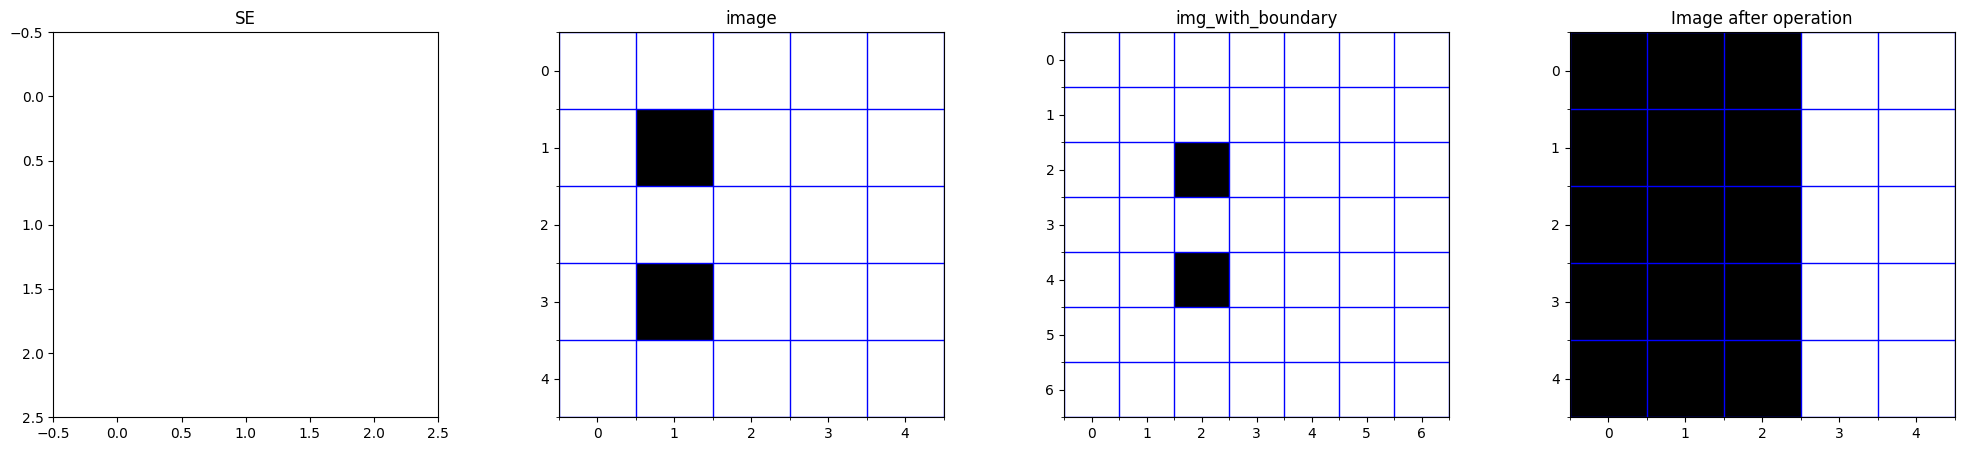
\includegraphics[width=\linewidth]{images/ef1_e1.png}
\\ 


\subsection{Erosion of f2 by vertical line of length 3 }
 The center of the SE would be the middle pixel since the given SE is a vertical line. The top and bottom border paddings of size 1 with the maximum value inside f2 (i.e. 5) are applied as indicated below as 'img\_with\_boundary'. Since f2 is saved in the gray-scale format, we replace the pixel where the SE's center is located with the minimum value got from its region during the erosion process.  \\
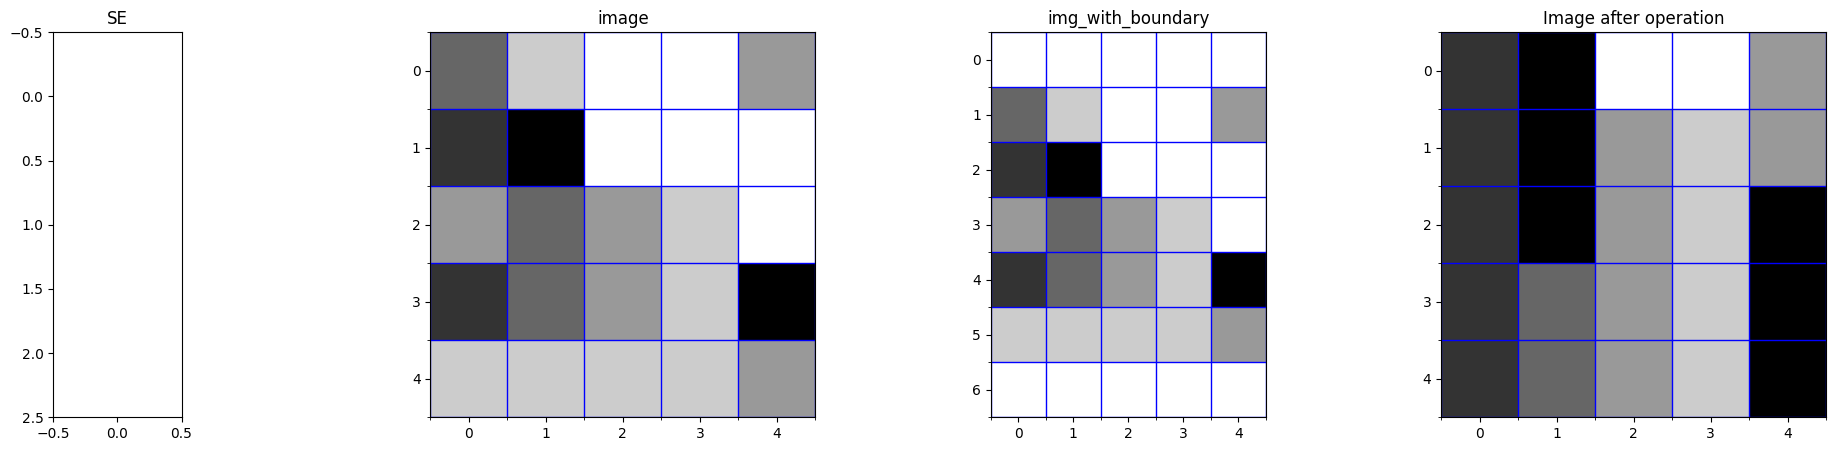
\includegraphics[width=\linewidth]{images/ef2_e2.png}
\\

\subsection{Erosion of f3 by horizontal line (-) of length 3}
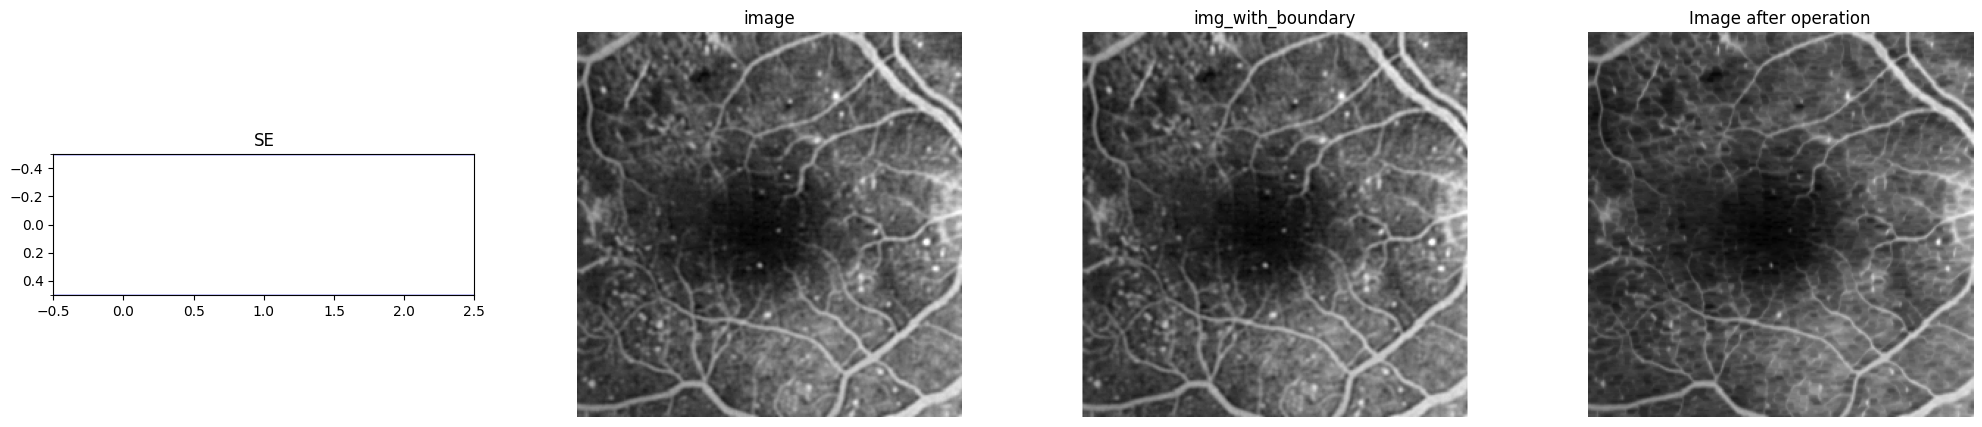
\includegraphics[width=\linewidth]{images/ef3_e2.png}
\\ 
\subsection{Erosion of f3 by square of size 5}
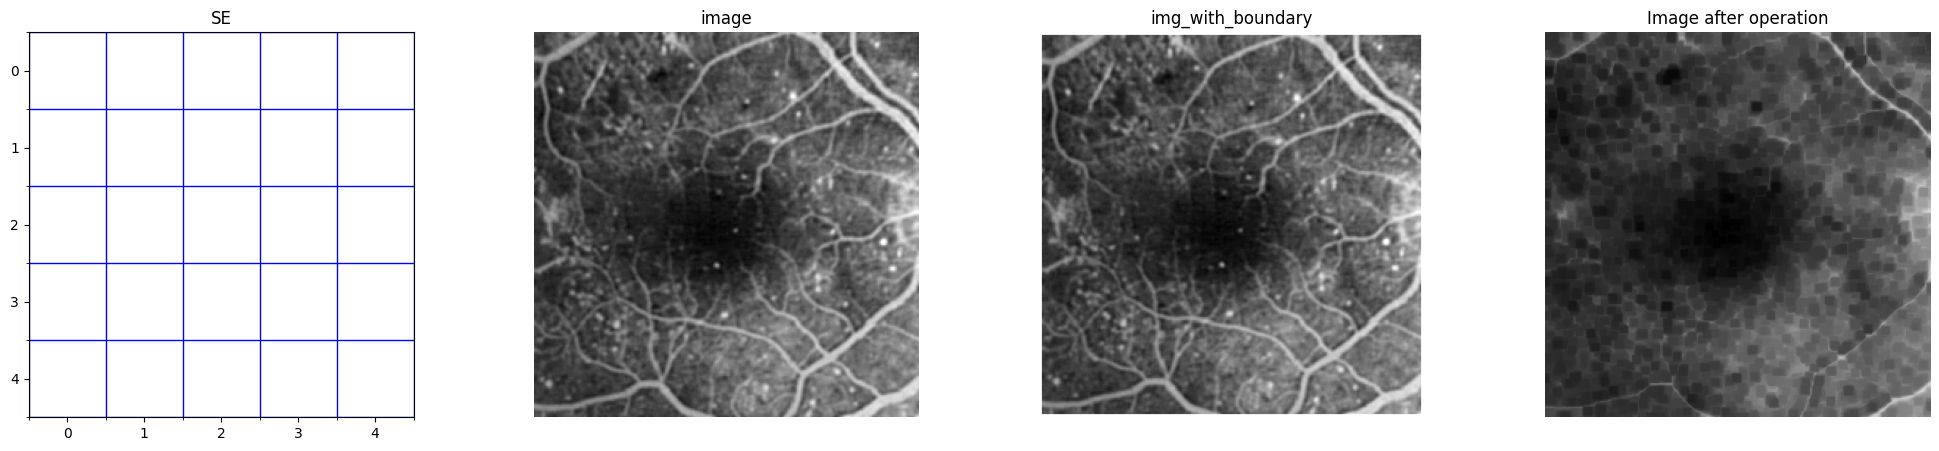
\includegraphics[width=\linewidth]{images/ef3_e3.png}
\\ 
\subsection{Erosion of f3 by backward diagonal (\textbackslash) of length 9}
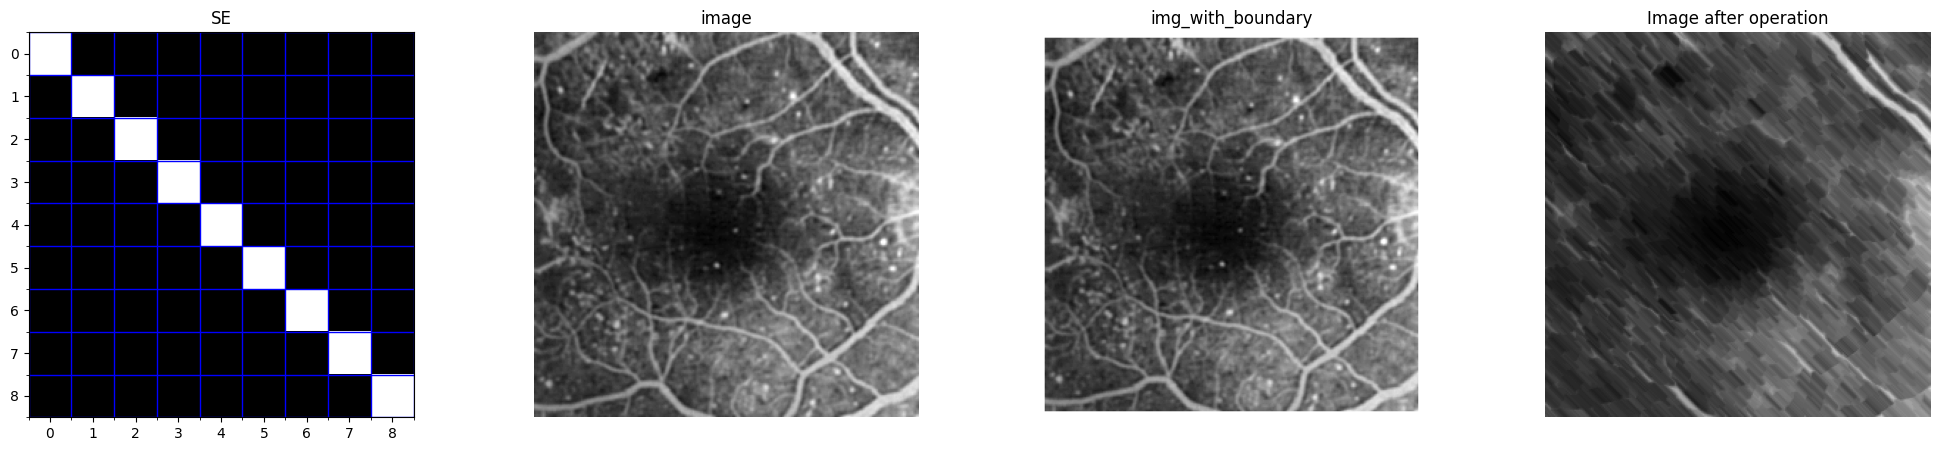
\includegraphics[width=\linewidth]{images/ef3_e4.png}
\\ 
\subsection{Erosion of f3 by forward diagonal (/) of length 9}
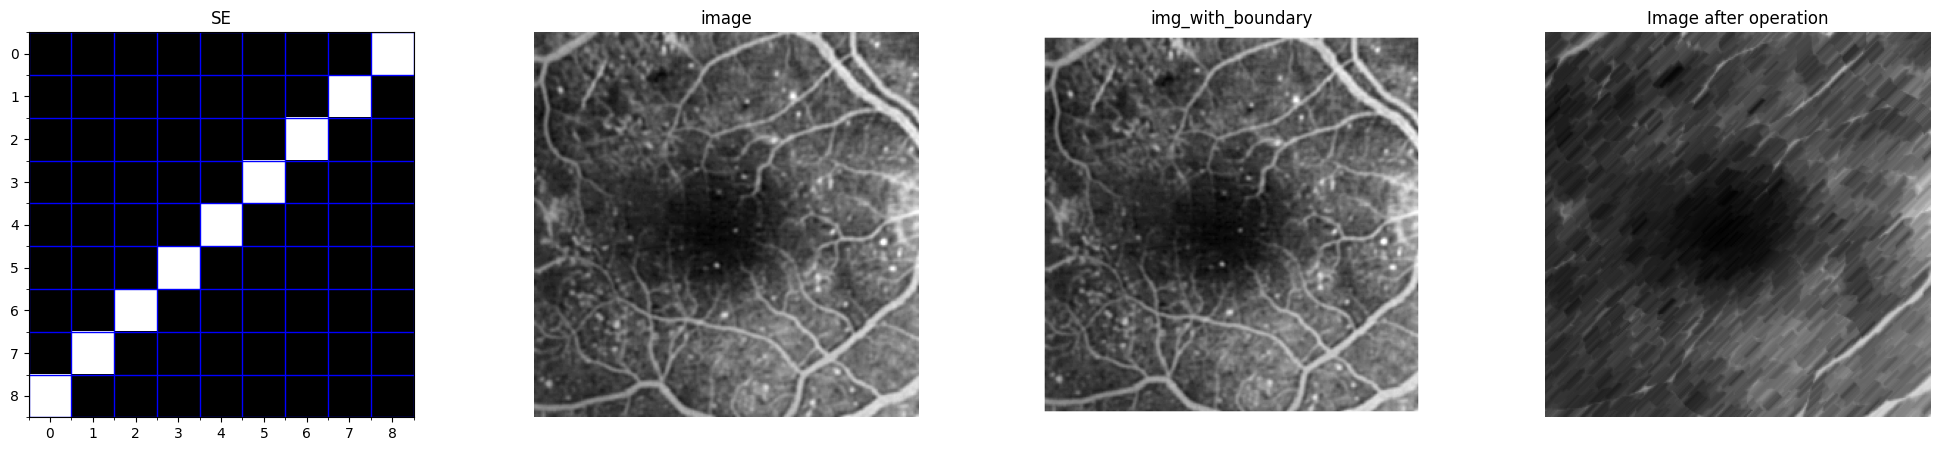
\includegraphics[width=\linewidth]{images/ef3_e5.png}
\\ 

\section{Dilation}
\subsection{Dilation of f3 by square of size 5}
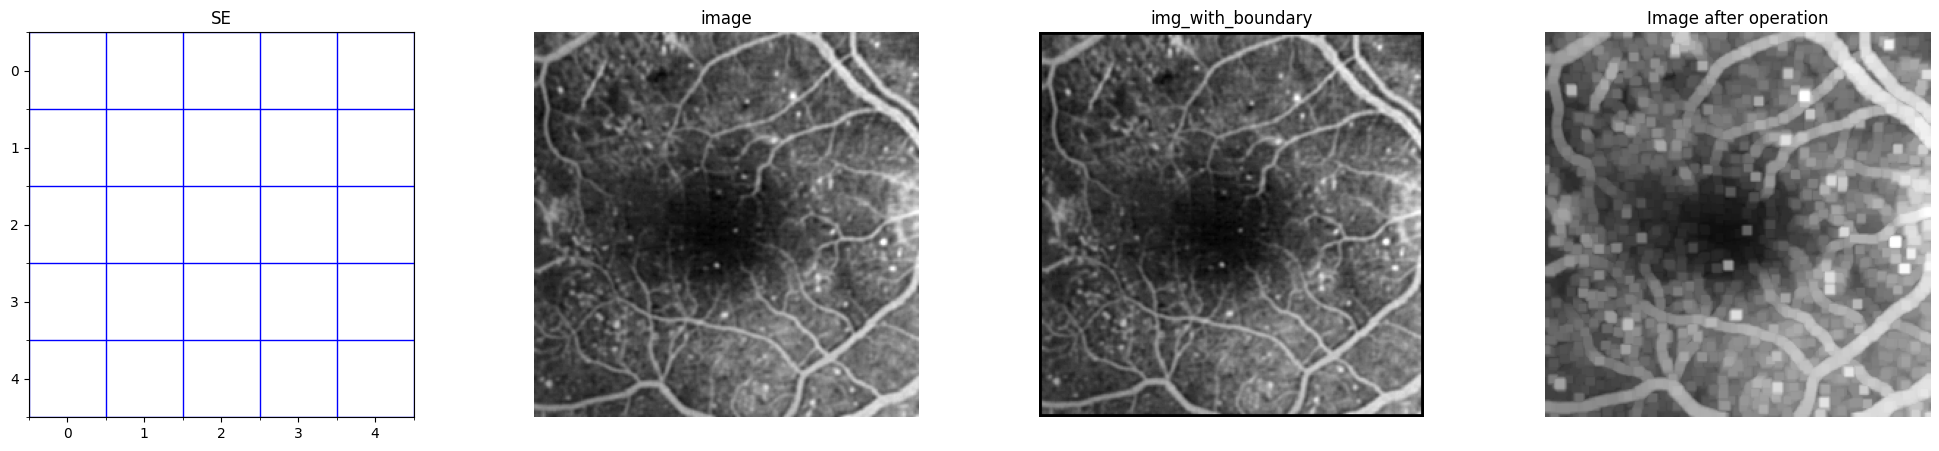
\includegraphics[width=\linewidth]{images/df3_d3.png}
\\ 

\subsection{Dilation of f3 by backward diagonal of length 9}
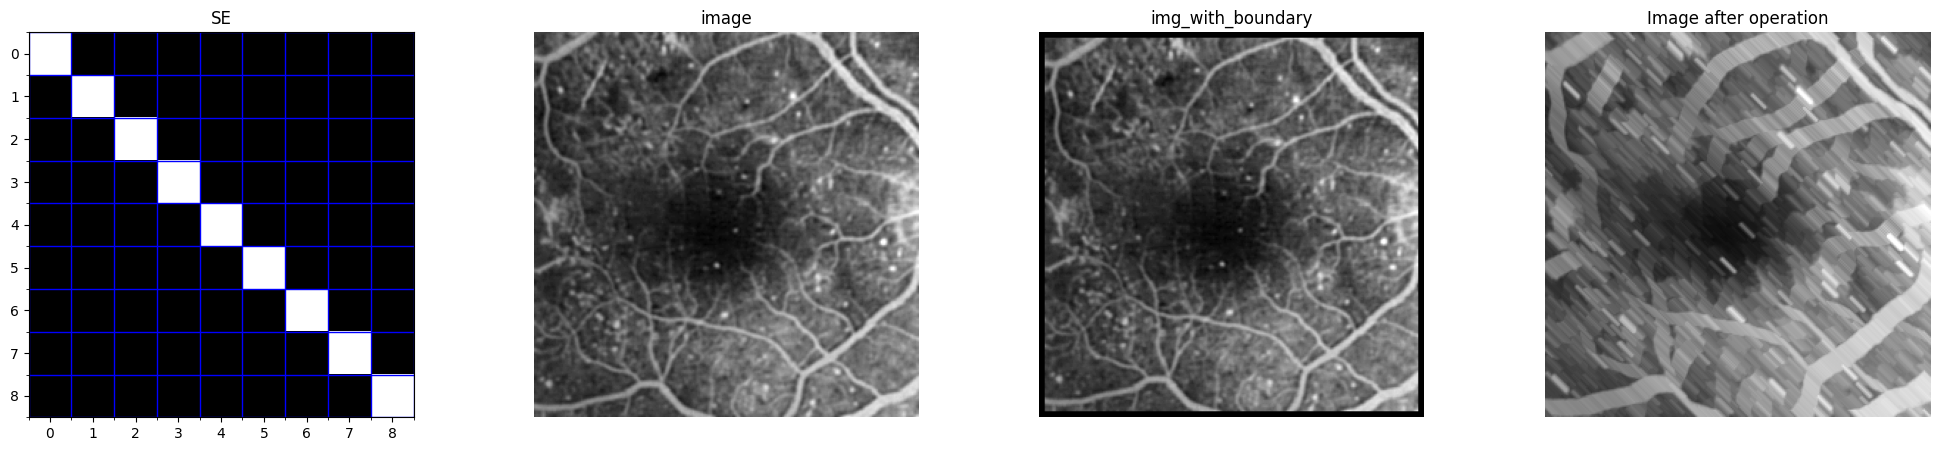
\includegraphics[width=\linewidth]{images/df3_d4.png}
\\ 

\subsection{Dilation of f3 by forward diagonal of length 9}
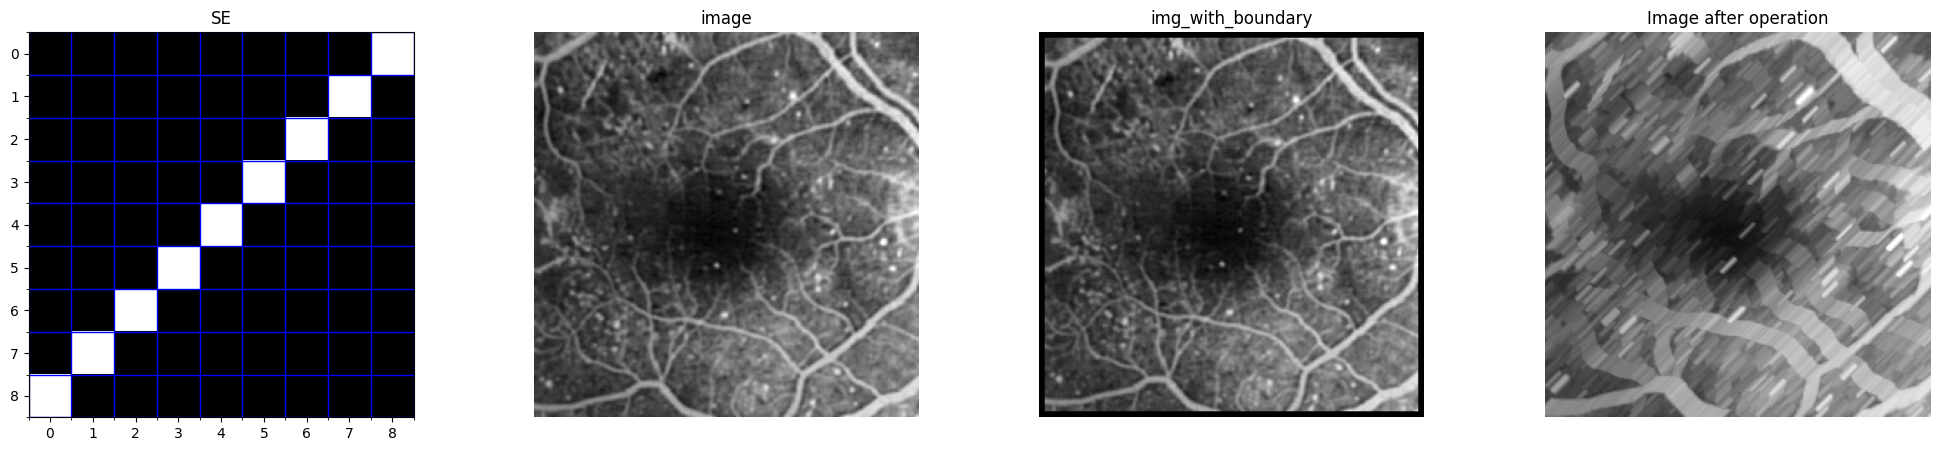
\includegraphics[width=\linewidth]{images/df3_d5.png}
\\ 

\subsection{Dilation of "ef3\_e3.txt" by square of size 5}
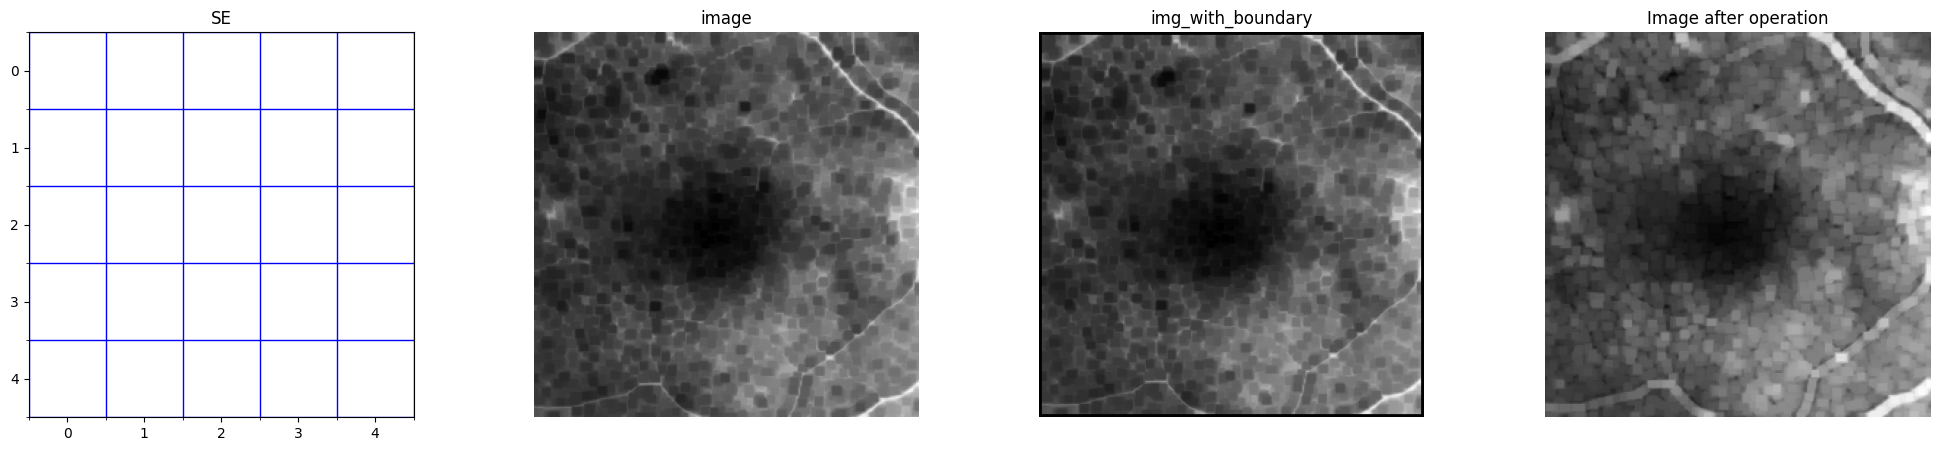
\includegraphics[width=\linewidth]{images/of3_o3.png}
\\ 

\subsection{Dilation of "ef3\_e4.txt" by backward diagonal of length 9}
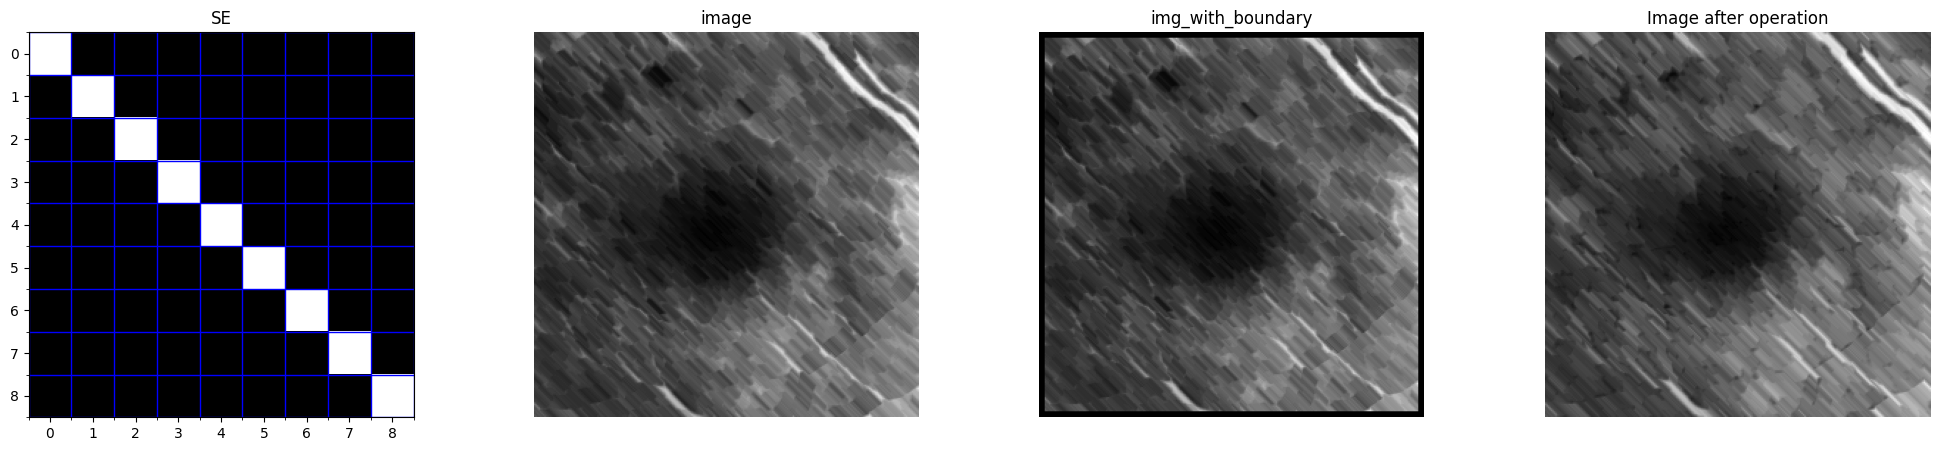
\includegraphics[width=\linewidth]{images/of3_o4.png}
\\ 

\section{Self Implementation}
\subsection{One self-chosen experiment with an asymmetric SE not containing the center}
\includegraphics[width=\linewidth]{images/}
\\
\subsection{At least three self-chosen images and experiments}
\subsubsection{Image 1}
\subsubsection{Image 2}
\subsubsection{Image 3}

\end{document}
